% Options for packages loaded elsewhere
\PassOptionsToPackage{unicode}{hyperref}
\PassOptionsToPackage{hyphens}{url}
%
\documentclass[
  11pt,
  a4paper,
]{article}
\usepackage{amsmath,amssymb}
\usepackage{lmodern}
\usepackage{iftex}
\ifPDFTeX
  \usepackage[T1]{fontenc}
  \usepackage[utf8]{inputenc}
  \usepackage{textcomp} % provide euro and other symbols
\else % if luatex or xetex
  \ifXeTeX
    \usepackage{zxjatype} 
    \usepackage[ipaex]{zxjafont}
  \fi
  \usepackage{unicode-math}
  \defaultfontfeatures{Scale=MatchLowercase}
  \defaultfontfeatures[\rmfamily]{Ligatures=TeX,Scale=1}
\fi
% Use upquote if available, for straight quotes in verbatim environments
\IfFileExists{upquote.sty}{\usepackage{upquote}}{}
\IfFileExists{microtype.sty}{% use microtype if available
  \usepackage[]{microtype}
  \UseMicrotypeSet[protrusion]{basicmath} % disable protrusion for tt fonts
}{}
\usepackage{xcolor}
\IfFileExists{xurl.sty}{\usepackage{xurl}}{} % add URL line breaks if available
\IfFileExists{bookmark.sty}{\usepackage{bookmark}}{\usepackage{hyperref}}
\hypersetup{
  pdftitle={Charitable Giving, Tax Reform, and Self-selection of Tax Relief: Evidence from South Korea},
  hidelinks,
  pdfcreator={LaTeX via pandoc}}
\urlstyle{same} % disable monospaced font for URLs
\usepackage[left=3cm,right=3cm,top=3cm,bottom=3cm]{geometry}

\usepackage{setspace}
\renewcommand{\baselinestretch}{1.5}
\usepackage{float}

\usepackage{longtable,booktabs,array}
\usepackage{threeparttable, threeparttablex, multirow}
\usepackage{calc} % for calculating minipage widths
% Correct order of tables after \paragraph or \subparagraph
\usepackage{etoolbox}
\makeatletter
\patchcmd\longtable{\par}{\if@noskipsec\mbox{}\fi\par}{}{}
\makeatother
% Allow footnotes in longtable head/foot
\IfFileExists{footnotehyper.sty}{\usepackage{footnotehyper}}{\usepackage{footnote}}
\makesavenoteenv{longtable}
\usepackage{graphicx}
\makeatletter
\def\maxwidth{\ifdim\Gin@nat@width>\linewidth\linewidth\else\Gin@nat@width\fi}
\def\maxheight{\ifdim\Gin@nat@height>\textheight\textheight\else\Gin@nat@height\fi}
\makeatother
% Scale images if necessary, so that they will not overflow the page
% margins by default, and it is still possible to overwrite the defaults
% using explicit options in \includegraphics[width, height, ...]{}
\setkeys{Gin}{width=\maxwidth,height=\maxheight,keepaspectratio}
% Set default figure placement to htbp
\makeatletter
\def\fps@figure{htbp}
\makeatother
\setlength{\emergencystretch}{3em} % prevent overfull lines
\providecommand{\tightlist}{%
  \setlength{\itemsep}{0pt}\setlength{\parskip}{0pt}}
\setcounter{secnumdepth}{5}
\newlength{\cslhangindent}
\setlength{\cslhangindent}{1.5em}
\newlength{\csllabelwidth}
\setlength{\csllabelwidth}{3em}
\newlength{\cslentryspacingunit} % times entry-spacing
\setlength{\cslentryspacingunit}{\parskip}
\newenvironment{CSLReferences}[2] % #1 hanging-ident, #2 entry spacing
 {% don't indent paragraphs
  \setlength{\parindent}{0pt}
  % turn on hanging indent if param 1 is 1
  \ifodd #1
  \let\oldpar\par
  \def\par{\hangindent=\cslhangindent\oldpar}
  \fi
  % set entry spacing
  \setlength{\parskip}{#2\cslentryspacingunit}
 }%
 {}
\usepackage{calc}
\newcommand{\CSLBlock}[1]{#1\hfill\break}
\newcommand{\CSLLeftMargin}[1]{\parbox[t]{\csllabelwidth}{#1}}
\newcommand{\CSLRightInline}[1]{\parbox[t]{\linewidth - \csllabelwidth}{#1}\break}
\newcommand{\CSLIndent}[1]{\hspace{\cslhangindent}#1}
\ifLuaTeX
  \usepackage{selnolig}  % disable illegal ligatures
\fi

\title{Charitable Giving, Tax Reform, and Self-selection of Tax Relief: Evidence from South Korea}


      \usepackage{authblk}
                            \author[]{Hiroki Kato}
                                      \affil{Graduate School of Economics, Osaka University, Japan \thanks{vge008kh@stundent.econ.osaka-u.ac.jp}}
                                                    \author[]{Tsuyoshi Goto}
                                      \affil{Graduate School of Social Sciences, Chiba University, Japan}
                                                    \author[]{Youngrok Kim}
                                      \affil{Graduate School of Economics, Kobe University, Japan}
                              
\date{2021/08/10}


\begin{document}
\begin{spacing}{1}
  \maketitle
\end{spacing}
\begin{spacing}{1}
  \begin{abstract}
    This paper investigates the price elasticity of charitable giving utilizing South Korean tax reform in 2014, when the tax relief on charitable giving changed from tax deduction to tax credit. Although many research on the price elasticity of charitable giving implicitly assume that all of tax payers declare their tax relief on charitable giving, this paper considers the existence of declaration cost for tax reliefs on charitable giving.
    By estimating the ``intension-to-treat'' effect (ITT) of tax reform, the analysis shows that the giving price elasticity is about -1 in terms of both intensive and extensive margins. Furthermore, considering the declaration of charitable giving and exploiting the different declaration cost between wage earners and self-employed workers as instrument variable (IV), we estimate the effect of ``effective'' giving price on the donation. As a result, we find that the estimation about the ``effective'' price elasticity is almost the same for the baseline one in terms of both intensive and extensive margins. This implies that the effect from the declaration cost of charitable giving may be small.
    
            \noindent
    \textbf{Keywords}: Charitable giving, Giving price, Tax reform, South Korea, 
        
        \noindent
    \textbf{JEL Codes}: D91, I10, I18, 
        
  \end{abstract}
\end{spacing}

\hypertarget{introduction}{%
\section{Introduction}\label{introduction}}

In many countries, governments set a tax relief for charitable giving. This is because, if subsidizing charitable giving induces a large increase in donations, it is desirable for public good provision. As Saez (2004) shows, it is known that the price elasticity of charitable donations is a key parameter to evaluate the welfare implication. To evaluate the effect of tax relief, many empirical papers investigate the elasticity of charitable donations with respect to their tax price and find that the price elasticity is around -1 in terms of intensive margin, using the data from tax record (Almunia et al., 2020; Auten et al., 2002; Bakija and Heim, 2011; Fack and Landais, 2010; Randolph, 1995).

However, as Almunia et al. (2020) point out, the analysis based on tax record only captures the effect for tax payers who declare charitable tax deduction, while charitable donation may also be conducted by those who do not declare it. As Fack and Landais (2016) and Gillitzer and Skov (2018) suggest that tax payers incur some cost for the declaration of charitable tax deduction such as record-keeping costs and compliance cost, tax payers may not declare their charitable giving if the benefit of the declaration exceeds the cost of it. Therefore, Rehavi and Shack (2013) suggest that the estimated tax elasticity will be biased if the data used for the estimation only focuses on tax payers who declare charitable tax deduction.

Considering the issue of the declaration, this paper follows the literature of charitable donation and tax relief, and investigates the price elasticity of giving. To derive the elasticity, this paper utilize the South Korean (Korea hereafter) tax reform in 2014, from when the tax relief on charitable giving was conducted by tax credit, though tax deduction had been used before 2014.

The extant research mainly focuses on the tax reform within the regime of tax deduction (Almunia et al., 2020; Auten et al., 2002; Bakija and Heim, 2011; Randolph, 1995) or tax credit (Fack and Landais, 2010). However, there is no research which deal with the giving tax reform between the regime of tax deduction and tax credit as far as we know. Since the extant research focus on the tax reform within the scheme of tax deduction or tax credit, this paper firstly deals with the tax reform from tax deduction system to tax credit system.

The Korean tax reform in 2014 started to allow 15\% of the total amount of charitable giving as a tax credit for all taxpayers, which means that the giving price for 1 KRW donation is 0.85 KRW.\footnote{1 KRW is approximately 0.001 USD. In other words, 1 USD is about 1,000 KRW.} Since the giving price was determined according to the marginal tax rate of progressive income tax before 2014, this tax reform reduced the giving price for low income taxpayers while it increased the price for high income tax payers. Since the variation of giving price can be considered to be exogenous for taxpayers, we exploit this reform and conduct the difference-in-difference (DID) analysis following the extant research about the giving price elasticity.

Moreover, to overcome the issue of tax declaration, we use the Korean survey panel data called the National Survey of Tax and Benefit (NaSTaB) and estimate intention-to-treat (ITT) of tax relief for giving as a baseline analysis. Since NaSTaB data contains the data of charitable giving irrespective of declarations, the baseline analysis examine the ITT of tax relief on the all charitable giving.
As a result, our baseline estimation shows that the price elasticity of charitable giving in Korea is -0.59 \textasciitilde{} -1.01 for intensive margins and -1.17 \textasciitilde{} -1.48 for extensive margins.

However, the estimation of the ITT implicitly assumes that the donors can automatically enjoy tax relief although tax payers have to declare their charitable giving to receive tax relief. Therefore, as an alternative way, we calculate an ``effective'' giving price considering whether each tax payer declare tax relief or not. Since whether tax payers declare or not may be endogenous with the amount of charitable giving, to overcome this issue, we focus on the fact that wage earners can easily declare tax relief in their company while self-employed workers have to declare tax relief via tax agency in Korea. By utilizing this difference of declaration costs between wage earners and self-employed workers as an instrument variable (IV), we estimate the price elasticity using the effective giving price, and compare the estimation with the baseline estimation. As a result, we find that the results using the effective price are -0.94 \textasciitilde{} -1.16 in terms of intensive margin and -0.92 \textasciitilde{} -1.46 in terms of extensive margin, which is almost the same for the baseline results. Since the estimated results are in line with the extant research, the result implies that the effect from the declaration cost may not so large.

This paper contributes the literature about the charitable giving tax system for the following points. Firstly, this paper considers the price elasticity of charitable giving using the effective giving price, although most of papers assume that the giving price applied for the charitable giving is the cheapest ``applicable'' giving price for each tax payer. As a result, although Rehavi and Shack (2013) suggest that the estimations using the effective price and the applicable price should be very different, our results suggest that the bias coming from the difference of the estimations may be small. Moreover, since our robustness checks to control the manipulations for giving price and intertemporal income shifting show more different results from the baseline ones than the results considering the declaration issue, the results implies that the bias from the declaration issue may be considerably small.

Secondly, by using the survey data, which cannot be manipulated, we could consider the sample of low-income household. The research in this literature typically use the tax return data, the main part of which is the data about wealthy people. Since our data is based on survey, which reflects the income distribution of population, we believe that we can estimate the giving price elasticity of population more precisely. Moreover, the usage of survey data is important for the estimation of the price elasticity in terms of the extensive margin since the propensity of donation by low-income households would be be less than high-income households.

Thirdly, this paper is the first paper to examine the giving price elasticity in a non-Western country. While the giving behavior may be affected by the cultural matter such as the religious belief, the estimated price elasticity in this paper is in line with the result of the extant papers.

This paper consist of seven sections. Section 2 and 3 respectively explain the institutional background and data. Section 4 explains the estimation method. Section 5 deals with the analysis of price elasticity using the applicable giving price and section 6 shows the analysis using the effective giving price. Section 7 concludes.

\hypertarget{institutional-background}{%
\section{Institutional background}\label{institutional-background}}

In this section, we describe the income tax relief for charitable giving in Korea and used dataset.

\hypertarget{tax-relief-for-charitable-giving-by-tax-deduction-and-tax-credit}{%
\subsection{Tax relief for charitable giving by tax deduction and tax credit}\label{tax-relief-for-charitable-giving-by-tax-deduction-and-tax-credit}}

In the South Korea, the tax policy about charitable giving drastically changed in 2014. Before then, tax relief of charitable giving was provided by tax deduction while, from 2014, tax relief by tax credit was introduced instead of tax deduction.

The tax deduction and tax credit may have different effects on giving behavior. This subsection summarize the difference of tax deduction and tax credit.
Consider that a household has a choice between private consumption (\(x_i\)) and charitable giving (\(g_i\)). Let \(y_i\) be pre-tax total income.
Then, the budget constraint is
\begin{align}
    x_i + g_i = y_i − R_iK - R_iT_i(y_i, g_i) - (1-R_i)T_i(y_i).
\end{align}
\(T_i\) is tax amount which depends on the pre-tax income and charitable giving.
\(R_i\) is the dummy which takes 1 if \(i\) declares the tax relief and 0 otherwise. \(K\) is a cost for the declaration of charitable giving, which may not be monetary cost but is converted to pecuniary terms.

Tax payers declare their charitable giving if its benefit exceeds its cost, which means

\begin{align}
R_i=\begin{cases}
1 \text{ if }T_i(y_i, g_i) - T_i(y_i)>K\\
0 \text{ if }T_i(y_i, g_i) - T_i(y_i)\le K.
\end{cases}
\end{align}

This means that the decision of declaration depends on \(y_i\), \(g_i\) and \(K\), where \(g_i\) is considered to be much easier for tax payers to adjust than the others.

On one hand, tax deduction reduces taxable income by giving. The amount of tax is

\begin{align}
    T_i(y_i, g_i) = \tau(y_i - g_i) \cdot (y_i - g_i),
\end{align}
or,
\begin{align}
    T_i(y_i) = \tau(y_i) \cdot (y_i),
\end{align}

where \(\tau(\cdot)\) is the income tax rate which is determined by \(y_i - g_i\) or \(y_i\).\footnote{\(\tau(\cdot)\) here is a function which shows the average tax rate, which is determined progressively. Since the price elasticity of giving shows the marginal and additional increment for one unit of price reduction increase, we use not average but marginal tax rate to construct the giving price following the literature. Usage of the function of the average tax rate here is for explanatory simplicity.} The budget constraint will be

\begin{align}
    x_i + [1 - R_i\tau(y_i - g_i)]g_i = [1 - R_i\tau(y_i - g_i)-(1-R_i)\tau(y_i)] y_i− R_iK.
\end{align}

Thus, the giving price compared to the price of private consumption is \(p_i^{d} \equiv 1 - R_i\tau(y_i - g_i)\) in tax deduction system. Since the giving price in tax deduction scheme varies depending on (1) the income level, (2) the amount of charitable giving, and (3) declaration of tax relief, it is endogenous to them, i.e.~(1), (2), and (3).

On the other hand, tax credit reduces tax amount directly, that is,

\[
    T_i = \tau(y_i)\cdot y_i - R_im g_i ,
\]

where \(m \in [0, 1]\) is the tax credit rate. Under the tax credit system, the budget constraint is

\begin{align}
    x_i + (1 - R_im) g_i = [1 - \tau(y_i)] y_i − R_iK.
\end{align}

Thus, the giving price of tax credit system will be \(p_i^c = 1 - R_im\), which is only dependent on the tax credit rate \(m\), which is exogenously determined by the government, and declaration \(R_i\).
Therefore, the giving price in the tax credit system would not be manipulated by donors except the declaration.

In the literature of giving tax relief, many papers implicitly assume that \(K=0\) and all tax payers should enjoy tax relief for charitable giving, i.e.~\(R_i=1\) for all \(i\).\footnote{As an exception, Rehavi and Shack (2013) and Almunia et al. (2020) respectively consider the declaration by using the survey data and the stractural estimation.} As a result, the observed amount of the charitable giving \(g_i\) may be different from the realized amount of the charitable giving \(g_i\).

To overcome this issue, we use two ways of estimations. In section 5, we assume \(R_i=1\) for all \(i\) following the extant research and estimate ITT as a baseline result. The difference between this analysis and the extant research is that the observed charitable giving \(g_i\) in the former is not limited to declared one, but \(g_i\) in the latter is limited to declared one. In section 6, we remove the assumption, that is \(R_i=1\), and \(R_i\) can be 0 or 1 depending on each \(i\), which is the difference from the extant research.

\begin{table}

\caption{\label{tab:tabTaxRate}Marginal Income Tax Rate}
\centering
\fontsize{9}{11}\selectfont
\begin{threeparttable}
\begin{tabular}[t]{lccccccc}
\toprule
Income/Year & 2008 & 2009 & 2010 \textasciitilde{} 2011 & 2012 \textasciitilde{} 2013 & 2014 \textasciitilde{} 2016 & 2017 & 2018\\
\midrule
(A) \textasciitilde{} 1200 & 8\% & 6\% & 6\% & 6\% & 6\% & 6\% & 6\%\\
\cmidrule{1-8}
(B) 1200 \textasciitilde{} 4600 & 17\% & 16\% & 15\% & 15\% & 15\% & 15\% & 15\%\\
\cmidrule{1-8}
(C) 4600 \textasciitilde{} 8800 & 26\% & 25\% & 24\% & 24\% & 24\% & 24\% & 24\%\\
\cmidrule{1-8}
(D) 8800 \textasciitilde{} 15000 &  &  &  &  & 35\% &  & 35\%\\
\cmidrule{1-1}
\cmidrule{6-6}
\cmidrule{8-8}
(E) 15000 \textasciitilde{} 30000 &  &  &  & \multirow{-2}{*}{\centering\arraybackslash 35\%} &  & \multirow{-2}{*}{\centering\arraybackslash 35\%} & 38\%\\
\cmidrule{1-1}
\cmidrule{5-5}
\cmidrule{7-8}
(F) 30000 \textasciitilde{} 50000 &  &  &  &  &  & 38\% & 40\%\\
\cmidrule{1-1}
\cmidrule{7-8}
(G) 50000 \textasciitilde{} & \multirow{-4}{*}{\centering\arraybackslash 35\%} & \multirow{-4}{*}{\centering\arraybackslash 35\%} & \multirow{-4}{*}{\centering\arraybackslash 35\%} & \multirow{-2}{*}{\centering\arraybackslash 38\%} & \multirow{-3}{*}{\centering\arraybackslash 38\%} & 40\% & 42\%\\
\bottomrule
\end{tabular}
\begin{tablenotes}
\item Notes: Marginal income tax rates applied from 2008 to 2018 are summarized. The income level is shown in terms of 10,000 KRW, which is approximately 10 United States dollars (USD) at an exchange rate of 1,000 KRW to one USD.
\end{tablenotes}
\end{threeparttable}
\end{table}

\hypertarget{korean-tax-reform-in-2014}{%
\subsection{Korean tax reform in 2014}\label{korean-tax-reform-in-2014}}

Korean tax system offers a tax relief for charitable giving in income tax. All tax payers have to declare their donation and submit the certificate of charitable giving to receive tax relief, while the taxiation method and the way of tax declaration are different for wage earners and self-employed workers. Wage earners pay income tax by withholding tax and declare tax relief for charitable giving via their company. Self-employed workers pay income tax by tax-return and declare tax relief when they submit tax return to the National Tax Service. Therefore, there is a difference of declaration cost of tax relief since self-employed workers have to retain the certificate until they submit tax return although wage earners can submit the certificate at any time.

In 2014, aiming at the relaxation of regressivity of giving price, the Korean government reformed tax system, where the tax credit was introduced instead of tax deduction. Since then, 15\% of the total amount of charitable giving has been allowed as a tax credit, which means that the giving price from 2014 is 0.85 KRW for each 1 KRW of donation irrelevant to the income level.

Summarizing this, compared to tax credit system, the high income household, whose (average) income tax rate is more than 15\%, get benefit from charitable giving under the tax deduction system. However, middle or low income households would enjoy tax relief in tax credit system more than tax deduction system. We exploit this policy change as an identification strategy.

\hypertarget{data}{%
\section{Data}\label{data}}

The National Survey of Tax and Benefit (hereafter, NaSTab) is an annual financial panel survey
implemented by The Korea Institute of Taxation and Finance
to study the tax burden of households and the benefits that households receive from the government.
The subjects of this survey are general households and household members living in 15 cities and provinces nationwide.
This survey is based on a face-to-face interview.\footnote{If it is difficult for investigators to meet subjects, another family member answers on behalf of him.}
The NaSTaB data is constructed as the subjects represent the population of Korean society.
This enables us to derive giving price elasticity of population without re-weighting samples, which is used in the extant research.
Moreover, note that subjects are not limited to the taxpayer or income earner reflecting the population.

In the analysis, we use data from 2013 to 2017 since we focus on the 2014 tax reform. This is because, as Table \ref{tab:tabTaxRate} shows, the giving price before 2014 was changed frequently and incorporating the data before 2012 captures the effects of another tax reform than the reform in 2014. Note that, since tax credit was introduced after 2014 and the credit rate was unchanged since 2014, the giving price does not depend on the income tax rate after 2014.
In addition, we exclude the subject of the sample, whose age is under 23, since they are not likely to have income or assets.

\begin{table}

\caption{\label{tab:SummaryCovariate}Descriptive Statistics}
\centering
\fontsize{9}{11}\selectfont
\begin{tabular}[t]{lcccccc}
\toprule
 & N & Mean & Std.Dev. & Min & Median & Max\\
\midrule
\addlinespace[0.3em]
\multicolumn{7}{l}{\textbf{Charitable Donations}}\\
\hspace{1em}Annual charitable giving (unit: 10,000KRW) & 67848 & 29.52 & 132.91 & 0.00 & 0.00 & 10000.00\\
\hspace{1em}Dummy of Donation > 0 & 67848 & 0.20 & 0.40 & 0.00 & 0.00 & 1.00\\
\addlinespace[0.3em]
\multicolumn{7}{l}{\textbf{Income, giving price, and tax report}}\\
\hspace{1em}Annual taxable labor income (unit: 10,000KRW) & 53269 & 1876.12 & 2700.97 & 0.00 & 900.00 & 91772.00\\
\hspace{1em}First giving price & 62877 & 0.86 & 0.04 & 0.62 & 0.85 & 0.94\\
\hspace{1em}Dummy of declaration of a tax relief & 12172 & 0.48 & 0.50 & 0.00 & 0.00 & 1.00\\
\addlinespace[0.3em]
\multicolumn{7}{l}{\textbf{Individual Characteristics}}\\
\hspace{1em}Age & 67848 & 51.35 & 15.81 & 24.00 & 50.00 & 104.00\\
\hspace{1em}Female dummy & 67848 & 0.53 & 0.50 & 0.00 & 1.00 & 1.00\\
\hspace{1em}Employee dummy & 42362 & 0.53 & 0.50 & 0.00 & 1.00 & 1.00\\
\hspace{1em}University graduate & 67842 & 0.41 & 0.49 & 0.00 & 0.00 & 1.00\\
\hspace{1em}High school graduate dummy & 67842 & 0.35 & 0.48 & 0.00 & 0.00 & 1.00\\
\hspace{1em}Junior high school graduate dummy & 67842 & 0.24 & 0.43 & 0.00 & 0.00 & 1.00\\
\bottomrule
\end{tabular}
\end{table}

Table \ref{tab:SummaryCovariate} shows summary statistics of our data.\footnote{Respondents answer the amount of donation for seven specific purposes last year. Seven specific purposes are policitical parties, educational organizations, social welfare organizations, organizations for culutre and art, religious groups, charity activies organaized by religious group, other purposes. We sum up the amount of donations, and consider it as the annual charitable giving.}
The first panel of this table shows variables about charitable giving.
The NaSTaB asks respondents to answer the amount of donation last year.
This is the first outcome variables.
Using this, we make a dummy taking 1 if respondent donated last year.
This is the second outcome variables to estimate the price effect on the decision of donations.
Table \ref{tab:SummaryCovariate} shows that
the average amount of donation is almost 300,000 KRW (300 USD),
and the proportion of donors is roughly 20\%.
Figure \ref{fig:SummaryOutcome} shows the time-series of two variables.
The blue line shows the average amount of donation among donors.
In each year, its value is nearly 1.5 million KRW (1,500 USD),
which is 7\% of average annual taxable income.
The gray bar shows the proportion of donors.
After the tax reform, the proportion of donors decreases by 2 percentage points.
After that, the proportion of donors is greter than 20\%.

\begin{figure}[t]

{\centering 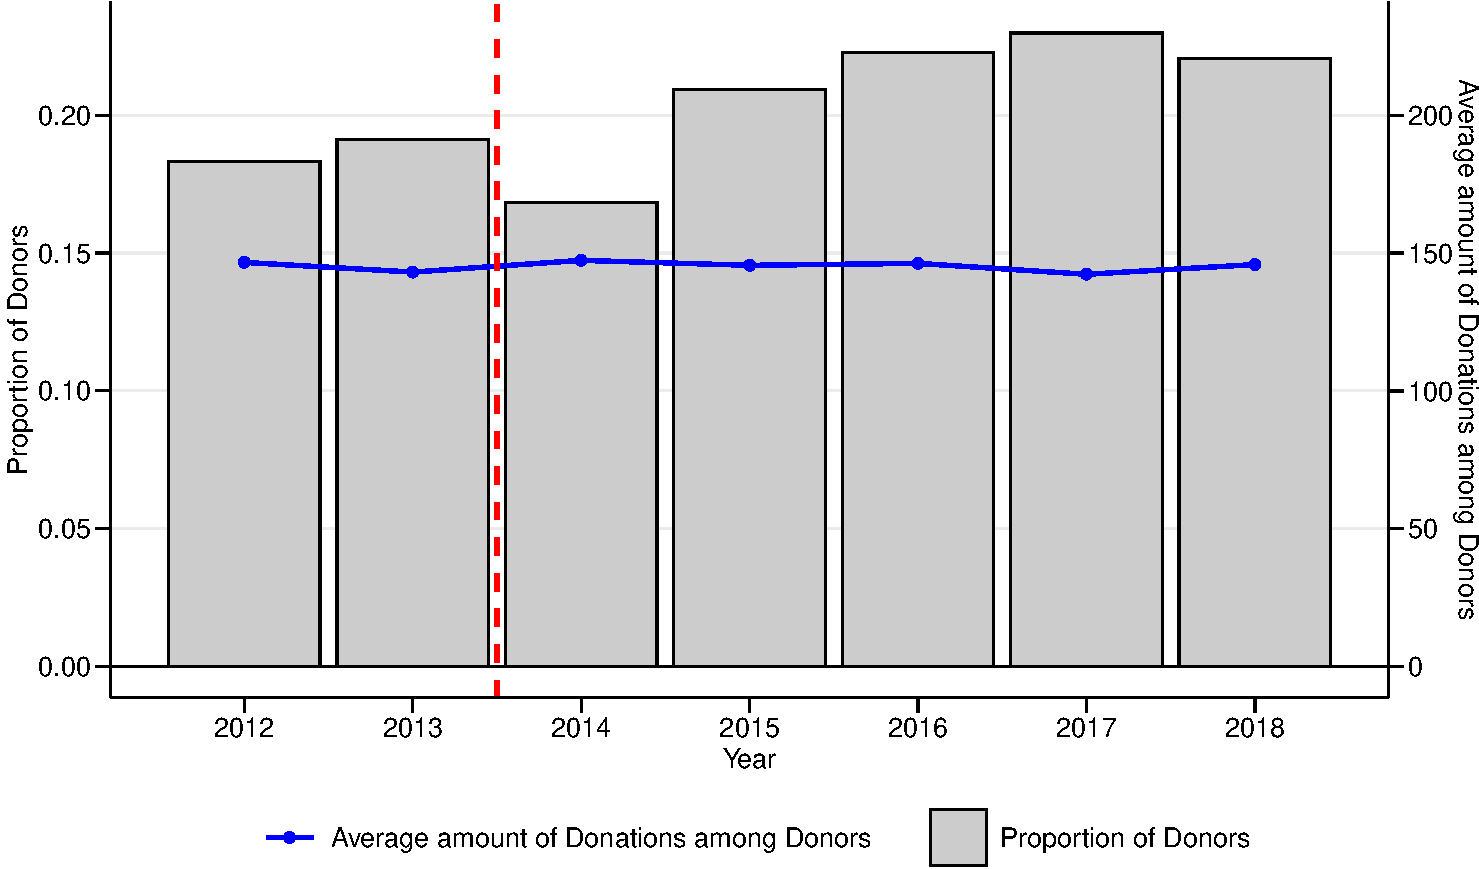
\includegraphics[width=1\linewidth]{C:/Users/vge00/Desktop/NASTAB/paper/draft_files/figure-latex/SummaryOutcome-1} 

}

\caption{Proportion of Donors and Average Donations among Donors. Notes: The left and right axises respectively mesure proportion of donors and the average amount donations among donors. Authors made this graph based on NasTaB data.}\label{fig:SummaryOutcome}
\end{figure}

The second panel of Table \ref{tab:SummaryCovariate} shows variables about income, tax report, and the giving price.
NaSTaB asks respondents to answer the annual labor income last year.
In our sample, the average annual taxable income is 18.76 million KRW (18,760 USD).
According to the National Tax Statistical Yearbook published by Korean National Tax Service,
the average annual taxable income is 32.77 million (32,770 USD) from 2012 to 2018
for employees who submitted the tax return.
Since our sample includes subjects with no labor income, such as housewives,
our sample mean of income is lower than the average income calculated by the public organizations.
In Figure \ref{fig:SummaryPriceChange},
the gray bars show the distribution of annual taxable income in 2013.
The income distribution is right-skewed.

Using this variable, we construct the giving price under the tax deduction system (2012 and 2013).\footnote{The giving price shown in Table \ref{tab:SummaryCovariate} is the \emph{first} giving price. The giving price can be manipulated by an amount of donation. To avoid this endogeneity, we use the giving price where the amount of donation is zero. We will discuss this issue in the next section.}
After the tax reform (after 2014), the giving price is 0.85 regardless of labor income.
as we explained in the section \ref{institutional-background}.
In Figure \ref{fig:SummaryPriceChange},
the blue line shows the giving price in 2012 and 2013,
while the red dashed line shows the giving price after 2014.
From this figure,
those whose annual income is less than 120,000,000 KRW (120,000 USD) in 2013 could receive benefit from the 2014 tax reform
because the tax reform decreases the giving price.
On the other hand,
those whose annual income is greater than 460,000,000 KRW (460,000 USD) in 2013 had a loss by the 2014 tax reform
since the tax reform increases the giving price.

The NaSTaB also asks respondents to answer whether they declared a tax relief of giving.
Although this variable is unique, the sample size is relatively small due to unanswering.
This survey investigates separately for the case of \emph{total} income (for example, business income, dividend income, rental income)
and the case of \emph{labor} income.
We make a dummy taking one if respondents applied for a total income deduction of giving
or a labor income deduction of giving.
Table \ref{tab:SummaryCovariate} shows the proportion of declaration is about 48\%.

\begin{figure}[t]

{\centering 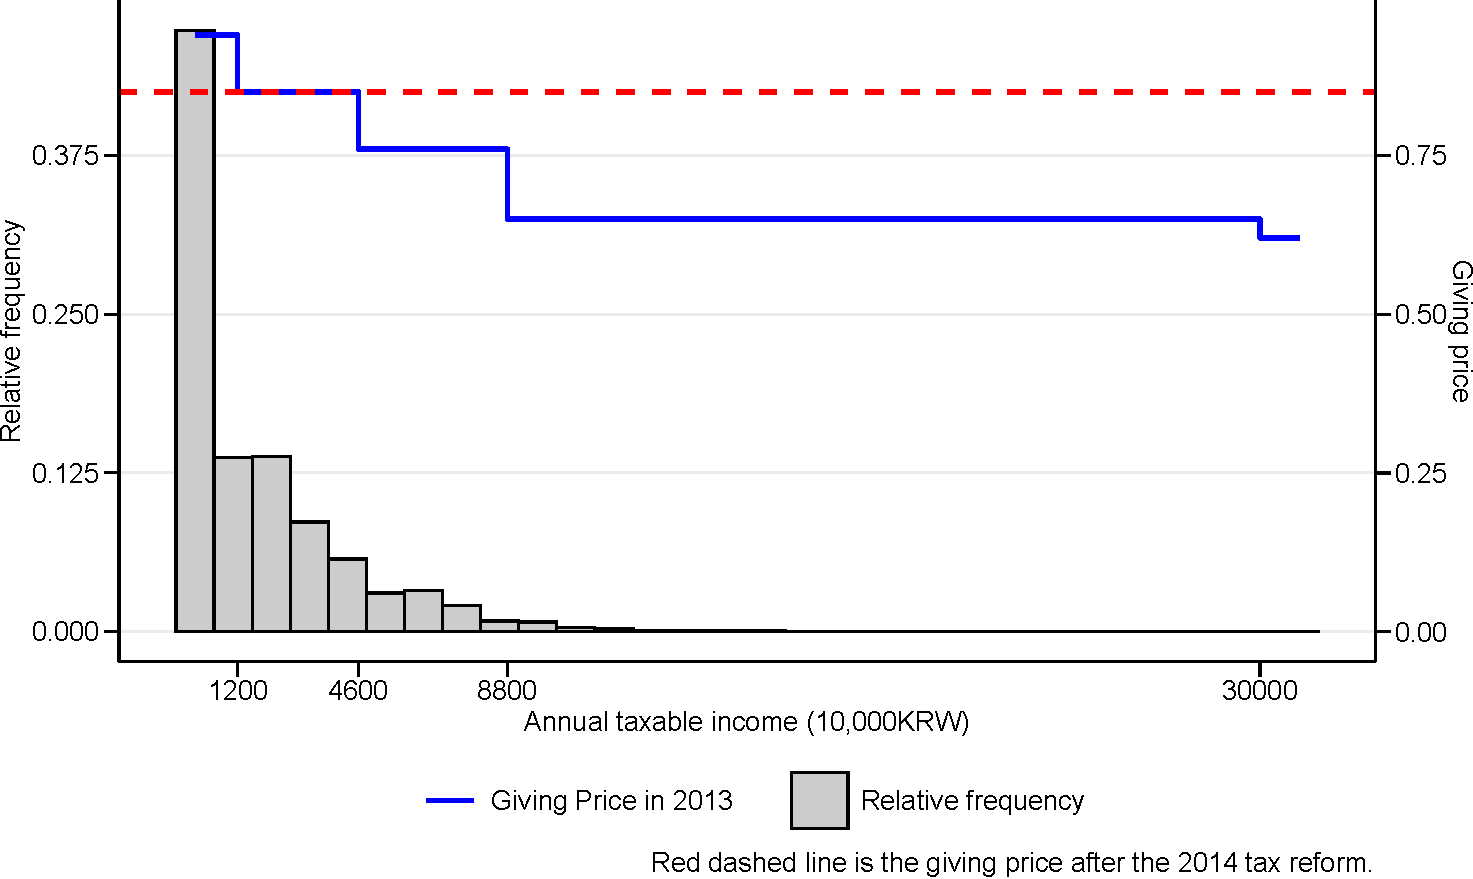
\includegraphics[width=0.85\linewidth]{C:/Users/vge00/Desktop/NASTAB/paper/draft_files/figure-latex/SummaryPriceChange-1} 

}

\caption{Income Distribution and Giving Price in 2013}\label{fig:SummaryPriceChange}
\end{figure}

\hypertarget{empirical-strategy}{%
\section{Empirical Strategy}\label{empirical-strategy}}

To estimate the giving price elasticity for intensive margin and extensive margin, we use DID analysis which exploit the fact that the giving price was unified in 2014 while the price was different for tax payers with different incomes.

Following Almunia et al. (2020), we estimate the giving price elasticity for intensive margin and extensive margin. The elasticity of intensive margin shows how much donors additionally donates reacting to the marginal increase of giving price, while the elasticity of extensive margin shows how much the probability to donate changes reacting to marginal increase of giving price.

\begin{equation}
    \ln g_{it} = \varepsilon^{int}_p R_{it} \ln p_{it} + \varepsilon^{int}_y \ln y_{it} 
    + X_{it}\beta +\mu_i +\iota_t +u_{it}. \label{eq:intensive}
\end{equation}

\(g_{it}, p_{it}\) and \(y_{it}\) respectively indicates the amount of giving, the giving price, and income of \(i\) in year \(t\).
\(R_{it}\) is a dummy taking one if individual \(i\) declared a tax relief in year \(t\).
\(\mu_i, \iota_t\) and \(u_{it}\) are individual fixed effect, year fixed effect, and the error term, respectively.
The individual fixed effect controls for time-invariant individual characteristics. The year fixed effect controls for events that affect all subjects at the same time. \(X_{it}\) is a vector of covariates, which consist of age, education, and gender, and their interaction terms between year fixed effect. The interaction terms between covariates and year fixed effect will control for events that affect subject with specific characteristics at the same time (Zeldow and Hatfield, 2021).

On the other hand,
the elasticity of extensive margin is estimated using the linear probability model such as

\begin{equation}
D_{it} =  \delta R_{it} \ln p_{it} +\gamma \ln y_{it} + X_{it}\beta +\mu_i  +\iota_t +v_{it}. \label{eq:extensive}
\end{equation}

\(D_{it}\) is a dummy variable taking 1 if individual \(i\) donates at year \(t\) and 0 otherwise.
Since we use the linear probability model,
the estimated coefficient \(\delta\) represents \(\hat{\delta} = \frac{\partial D_{it}}{\partial p_{it}} p_{it}\).
Also, the estimated coefficient \(\gamma\) represents \(\hat{\gamma} = \frac{\partial D_{it}}{\partial y_{it}} y_{it}\).
Thus, the implied extensive-margin price and income elasticity are calculated by
\(\hat{\delta}/\bar{D}\) and \(\hat{\gamma}/\bar{D}\), respectively,
where \(\bar{D}\) is sample average of outcome variable \(D_{it}\).

As shown in the section \ref{institutional-background},
the giving price \(p_{it}\) is defined as follows:

\begin{align}
  p_{it}(y_{it}, g_{it}) =
  \begin{cases}
    1 - \tau_t(y_{it} - g_{it})  \quad\text{if}\quad t < 2014  \\
    1 - m \quad\text{if}\quad t \ge 2014
  \end{cases}, \label{eq:price}
\end{align}
where \(\tau_t(\cdot)\) is average tax rate in year \(t\).

Our identification assumption is that the \emph{within} price variation is exogenous due to the fixed effect model.
From the equation \eqref{eq:price},
the within price variation comes from the 2014 tax reform, the within variation of giving \(g_{it}\) and income \(y_{it}\).
Moreover, by the equation \eqref{eq:intensive} and \eqref{eq:extensive},
the within price variation comes from tax report \(R_{it}\).
Since these three variables are self-selected,
we need to solve three potential endogeneity problems to hold our identification assumption.

As a benchmark, we estimate the equation \eqref{eq:intensive} and \eqref{eq:extensive},
assuming that \(R_{it} = 1\) for all \(i\) and \(t\).
This means that we see individuals who did not apply for a tax deduction as those who applied for a tax deduction.
In the context of treatment effect literature,
we can see the relative price of giving as a treatment assignment.
However, individuals can choose whether to receive this treatment by appling for a tax deduction.
Although assuming \(R_{it} = 1\) for all \(i\) and \(t\) can ignore this self-selection problem,
the estimates of price effect includes the \emph{true} price effect and effect of self-selection of a tax deduction.
this treatment effect is sometimes called the ``intention-to-treat'' effect (ITT).
Later, we relax this assumption, using the instrumental variable strategy.

Next, we deal with the possibility that the giving price is endogenous because
the taxpayer can reduce their giving price by reducing their amount of donation
and shifting themselves to the lower tax bracket in the tax deduction system.
Since this issue does not happen for the first unit of donation,
whose price (``first price'') cannot be changed by adjusting the donation,
we use this first price as the giving price in the estimation.
The first price is obtained by \(p^f_{it} = p_{it}(y_{it}, g_{it})\) evalueated at \(g_{it} = 0\).
As long as income \(y_{it}\) is exogenous, the within giving price \(p^f_{it}\) is also exogenous.
Thus, assuming income \(y_{it}\) is exogenous variable,
we first estimate the first-price elasticity with the equation \eqref{eq:intensive} and \eqref{eq:extensive}
which replace \(\ln p_{it}\) with \(\ln p^f_{it}\).
Moreover, we also estimate the last-price elasticity, using the first price \(p^f_{it}\) as an instrument.

We can justify the first price method, assuming that income is exogenous.
The second approach relaxes this assumption.
Under the tax deduction system,
the change of income have effects on both donations through the income effect
and the giving price through the marginal tax rate (Auten et al., 2002; Bakija and Heim, 2011; Randolph, 1995).
Therefore, following Bakija and Heim (2011),
we employ lagged values of taxable income and
construct a variable for the change in the first price of giving as following:

\begin{align}
  \Delta^k \ln p_{it} = \ln \left(\frac{p^f_{it}(y_{it-k})}{p^f_{it-k}(y_{it-k})}\right),
  \label{eq:laggedp}
\end{align}

The numerator is the first price that individual \(i\) would have faced in year \(t\)
if she had declared her year \((t - k)\) taxable income at that year.
By fixing the income at year \(t - k\), this variable isolates changes in price from income responses to the tax reform.
Note that this problem does not happen for the tax credit system, where the giving price is the same across all individuals.

Using this lagged variable, we estimate the \(k\)-th difference model formualted as follows:

\begin{align}
  \Delta^k \ln g_{it} = \varepsilon_p \Delta^k \ln p_{it} + \varepsilon_y \Delta^k \ln y_{it} 
  + \Delta^k X_{it} \beta + \mu_i + \iota_t + v_{it}, \label{eq:kdiff}
\end{align}
where \(\Delta^k \ln g_{it} = \ln g_{it} - \ln g_{it-k}\),
and \(\Delta^k \ln y_{it} = \ln y_{it} - \ln y_{it-k}\).
The variation of \(\Delta^k \ln p_{it}\) comes from the tax reform because we fix the annual income at year \(t - k\).
Therefore, we can interpret this coefficient as the giving price elasticity due to the tax reform.
Note that we do not estimate the extensive-margin elasticity because it is hard to interpret this estimation equation when we use \(\Delta^k D_{it}\) as an outcome variable.

\hypertarget{price-and-income-elasticitiy-itt-approach}{%
\section{Price and Income Elasticitiy: ITT Approach}\label{price-and-income-elasticitiy-itt-approach}}

In this section, as a benchmark, we first report the price effect on donations, using the ITT approach.
Reducing the relative price of giving through a tax deduction includes self-selection of declaration.
The ITT approach sees respondents who did not declare a tax relief in a specific year as those who applied for it.
In our main results, we report estimation results of price effect, using the first price method.
As robustness, we report the last price effect using the first price as an instrumental variable,
the first price effect with short-period panel to focus on the 2014 tax reform more precisely,
and the \(k\)-th difference model to avoid the problem that income affects the giving price.

\hypertarget{results}{%
\subsection{Results}\label{results}}

Before the estimation of giving price elasticities for intensive and extensive margin,
we estimate the elasticity without distinguishing them.
We call this elasticity overall elasticity.
Table \ref{tab:MainOverall} shows estimation results of overall elasticity.
Column (1) is the baseline estimation, which includes individual and time fixed effects.
The price elasticity is roughly -1, which is statistically significantly different from zero.
This implies that a 1\% increase of giving price raises charitable giving by 1\%.
This result is in line with previous researches which focuses on Western countries.
The income elasticity is about 5.3, which is statistically significantly different from zero.
This implies that a 1\% increase of annual income raises charitable giving by 5.3\%.
The remaining four columns control for events that affect subjects with specific characteristics at the same time.
As a result, the price elasticity is more elastic than the baseline result.
The price elasticity lies between -1.3 and -1.1.
On the other hand, the income elasticity is less elastic than the baseline result.
The income elasticity lies between -5.1 and -4.9.

\begin{table}

\caption{\label{tab:MainOverall}Overall Elasticity of First Price}
\centering
\fontsize{9}{11}\selectfont
\begin{threeparttable}
\begin{tabular}[t]{lccccc}
\toprule
 & (1) & (2) & (3) & (4) & (5)\\
\midrule
ln(giving price) & -1.072*** & -1.264*** & -1.291*** & -1.114*** & -1.241***\\
 & (0.202) & (0.213) & (0.230) & (0.229) & (0.227)\\
ln(annual taxable income) & 5.393*** & 5.080*** & 5.047*** & 5.116*** & 4.946***\\
 & (0.970) & (0.964) & (0.964) & (0.966) & (0.949)\\
Individual FE & Y & Y & Y & Y & Y\\
Time FE & Y & Y & Y & Y & Y\\
Age & N & Y & Y & Y & Y\\
Year x Education & N & N & Y & Y & Y\\
Year x Gender & N & N & N & Y & Y\\
Year x Resident Area & N & N & N & N & Y\\
N & 53269 & 53269 & 53267 & 53267 & 53267\\
Adjusted R-squared & 0.526 & 0.526 & 0.526 & 0.527 & 0.530\\
\bottomrule
\end{tabular}
\begin{tablenotes}
\item Notes: $^{*}$ $p < 0.1$, $^{**}$ $p < 0.05$, $^{***}$ $p < 0.01$. Standard errors are clustered at individual level. When controlling age, we alson include its squared term.
\end{tablenotes}
\end{threeparttable}
\end{table}

Table \ref{tab:MainIntensive} shows the intensive-margin elasticities.
Compared to the overall elasticity, the price and income elasticities are less elastic.
Controlling individual and time fixed effects,
the price and income elasticity are about -0.6 and about 2, respectively,
which are statistically significantly different from zero (See column (1)).
Moreover, when we include the interaction term between individual characteristics and year dummies,
these values vary.
The price elasticity lies between -1.1 and -0.8,
and the income elasticity lies between 1.4 and 1.6.
Anyway, we conclude that the amount of donations is insensitive to the giving price among donors.

\begin{table}

\caption{\label{tab:MainIntensive}Intensive-Margin Elasticity of First Price}
\centering
\fontsize{9}{11}\selectfont
\begin{threeparttable}
\begin{tabular}[t]{lccccc}
\toprule
 & (1) & (2) & (3) & (4) & (5)\\
\midrule
ln(giving price) & -0.593*** & -0.838*** & -1.016*** & -0.893*** & -0.904***\\
 & (0.203) & (0.212) & (0.232) & (0.243) & (0.249)\\
ln(annual taxable income) & 2.015*** & 1.562** & 1.445** & 1.528** & 1.571**\\
 & (0.675) & (0.655) & (0.647) & (0.651) & (0.653)\\
Individual FE & Y & Y & Y & Y & Y\\
Time FE & Y & Y & Y & Y & Y\\
Age & N & Y & Y & Y & Y\\
Year x Education & N & N & Y & Y & Y\\
Year x Gender & N & N & N & Y & Y\\
Year x Resident Area & N & N & N & N & Y\\
N & 11637 & 11637 & 11637 & 11637 & 11637\\
Adjusted R-squared & 0.675 & 0.675 & 0.676 & 0.676 & 0.678\\
\bottomrule
\end{tabular}
\begin{tablenotes}
\item Notes: $^{*}$ $p < 0.1$, $^{**}$ $p < 0.05$, $^{***}$ $p < 0.01$. Standard errors are clustered at individual level. When controlling age, we alson include its squared term.
\end{tablenotes}
\end{threeparttable}
\end{table}

Table \ref{tab:MainExtensive} shows the extensive-margin elasticities.
As a result of overall elasticities and the intensive-margin elasticities,
we expect that the extensive-margin price and income elasticity is more elastic than the overall elasticities.
In column (1), the coefficient of logged giving price and logged annual income are -0.257 and 1.175 respectively,
which are statistically significantly different from zero.
Due to the linear probability model,
the coefficient of logged giving price and logged income represents the lower bound of price and income elasticity, respectively.
When we evaluate the price elasticity at the sample mean of \(D_{it}\),
the implied price elasticity is -1.264, which is slightly more elastic than the overall one.
Also, we evaluate the income elasticity at the sample mean of the outcome.
The implied income elasticity is 5.778, which is slightly more elastic than the overall one.
Although the implied price and income elasticity vary with covariates,
the results are in line with our expectations.
Thus, the decision of donations is sensitive to the giving price and annual income.

In summary, our first conclusion is that
the decision of donations is sensitive to the giving price,
and the amount of donations is insensitive to the giving price once they decide to donate.
In the next subsection, we check the robustness of our first conclusion, using three methods.

\begin{table}

\caption{\label{tab:MainExtensive}Extensive-Margin Elasticity of First Price}
\centering
\fontsize{9}{11}\selectfont
\begin{threeparttable}
\begin{tabular}[t]{lccccc}
\toprule
 & (1) & (2) & (3) & (4) & (5)\\
\midrule
ln(giving price) & -0.257*** & -0.288*** & -0.273*** & -0.237*** & -0.267***\\
 & (0.046) & (0.048) & (0.052) & (0.052) & (0.051)\\
ln(annual taxable income) & 1.175*** & 1.124*** & 1.125*** & 1.139*** & 1.102***\\
 & (0.223) & (0.223) & (0.223) & (0.224) & (0.220)\\
 &  &  &  &  & \\
Implied price elasticity & -1.176*** & -1.320*** & -1.250*** & -1.086*** & -1.221***\\
 & (0.210) & (0.221) & (0.239) & (0.238) & (0.235)\\
Implied income elasticity & 5.379*** & 5.145*** & 5.148*** & 5.212*** & 5.045***\\
 & (1.023) & (1.021) & (1.023) & (1.024) & (1.005)\\
Individual FE & Y & Y & Y & Y & Y\\
Time FE & Y & Y & Y & Y & Y\\
Age & N & Y & Y & Y & Y\\
Year x Education & N & N & Y & Y & Y\\
Year x Gender & N & N & N & Y & Y\\
Year x Resident Area & N & N & N & N & Y\\
N & 53269 & 53269 & 53267 & 53267 & 53267\\
Adjusted R-squared & 0.458 & 0.458 & 0.458 & 0.458 & 0.462\\
\bottomrule
\end{tabular}
\begin{tablenotes}
\item Notes: $^{*}$ $p < 0.1$, $^{**}$ $p < 0.05$, $^{***}$ $p < 0.01$. Standard errors are clustered at individual level. When controlling age, we alson include its squared term. The implied extensive-marign price elasticity is evaluated at the sample mean of $D_{ijt}$.
\end{tablenotes}
\end{threeparttable}
\end{table}

\hypertarget{robustness-check}{%
\subsection{Robustness Check}\label{robustness-check}}

\emph{Last Price Elasticity.}
The first robustness check estimates the last price elasticity using the first price of giving as an instrument.
Our main results show that first price elasticity to avoid the problem that giving price depends on an amount of giving.
However, the first price elasticity is not realistic because people face the last marginal price when deciding on an amount of donation.
Thus, we estimate the last price elasticity, using the first price as an instrumental variable.
The last giving price is strongly correlated with the first one because
major observation units are observed when the tax credit system is implemented,
and the last price is equivalent to the first one in the case of the tax credit system.\footnote{In fact, in any specifications, the coefficient of the first price is greater than 0.952, and its F-statistics is greater than 6425.96. We do not show the first stage results of the panel IV using the first price as an insrument.}
Our estimates of the last price effect are not caused by a weak instrument problem.
As a result, the intensive-margin elasticity of the last price takes a similar value to the case of the first price, while
the overall elasticity and extensive-margin elasticity of the last price are more elastic than the case of the first price.
Table \ref{tab:LastOverall} shows the overall last price elasticity.
Compared to the main results, the last price elasticity is more elastic.
The absolute value of the estimated coefficient is larger than 2.4,
which is statistically significantly different from zero.
This implies that a 1\% increase of last price decreases charitable contributions by 2.4\% or more.
Table \ref{tab:LastIntensive} and \ref{tab:LastExtensive} shows
the intensive-margin and extensive-margin last price elasticity.
the intensive-margin last price elasticity is a similar value to the main results.
Its absolute value lies between 0.89 and 1.2.
These results are statistically different from zero.
About the extensive-margin elasticities,
the coefficient of logged last price, which represents the lower bound of last price elasticity,
lies between -0.63 and -0.59.
The implied last price elasticity evaluated at the sample mean of \(D_{it}\) is roughly -3.
These results are statistically significantly different from zero, and more elastic than the first price elasticity.

\begin{table}

\caption{\label{tab:LastOverall}Overall Elasticity of Last Price}
\centering
\fontsize{9}{11}\selectfont
\begin{threeparttable}
\begin{tabular}[t]{lccccc}
\toprule
 & (1) & (2) & (3) & (4) & (5)\\
\midrule
ln(last giving price) & -2.421*** & -2.536*** & -2.750*** & -2.529*** & -2.650***\\
 & (0.204) & (0.216) & (0.233) & (0.231) & (0.229)\\
ln(annual taxable income) & 5.258*** & 5.072*** & 4.981*** & 5.058*** & 4.910***\\
 & (0.961) & (0.961) & (0.959) & (0.961) & (0.948)\\
Individual FE & Y & Y & Y & Y & Y\\
Time FE & Y & Y & Y & Y & Y\\
Age & N & Y & Y & Y & Y\\
Year x Education & N & N & Y & Y & Y\\
Year x Gender & N & N & N & Y & Y\\
Year x Resident Area & N & N & N & N & Y\\
N & 52304 & 52304 & 52302 & 52302 & 52302\\
Adjusted R-squared & 0.529 & 0.529 & 0.529 & 0.530 & 0.533\\
\bottomrule
\end{tabular}
\begin{tablenotes}
\item Notes: $^{*}$ $p < 0.1$, $^{**}$ $p < 0.05$, $^{***}$ $p < 0.01$. Standard errors are clustered at individual level. The instumental variable is the first giving price in year $t$. When controlling age, we alson include its squared term.
\end{tablenotes}
\end{threeparttable}
\end{table}

\begin{table}

\caption{\label{tab:LastIntensive}Intensive-Margin Elasticity of Last Price}
\centering
\fontsize{9}{11}\selectfont
\begin{threeparttable}
\begin{tabular}[t]{lccccc}
\toprule
 & (1) & (2) & (3) & (4) & (5)\\
\midrule
ln(last giving price) & -0.898*** & -0.961*** & -1.197*** & -0.998*** & -1.074***\\
 & (0.271) & (0.271) & (0.307) & (0.325) & (0.332)\\
ln(annual taxable income) & 2.024*** & 1.638** & 1.460** & 1.530** & 1.572**\\
 & (0.694) & (0.678) & (0.667) & (0.670) & (0.667)\\
Individual FE & Y & Y & Y & Y & Y\\
Time FE & Y & Y & Y & Y & Y\\
Age & N & Y & Y & Y & Y\\
Year x Education & N & N & Y & Y & Y\\
Year x Gender & N & N & N & Y & Y\\
Year x Resident Area & N & N & N & N & Y\\
N & 10672 & 10672 & 10672 & 10672 & 10672\\
Adjusted R-squared & 0.671 & 0.671 & 0.672 & 0.672 & 0.674\\
\bottomrule
\end{tabular}
\begin{tablenotes}
\item Notes: $^{*}$ $p < 0.1$, $^{**}$ $p < 0.05$, $^{***}$ $p < 0.01$. Standard errors are clustered at individual level. The instumental variable is the first giving price in year $t$. When controlling age, we alson include its squared term.
\end{tablenotes}
\end{threeparttable}
\end{table}

\begin{table}

\caption{\label{tab:LastExtensive}Extensive-Margin Elasticity of Last Price}
\centering
\fontsize{9}{11}\selectfont
\begin{threeparttable}
\begin{tabular}[t]{lccccc}
\toprule
 & (1) & (2) & (3) & (4) & (5)\\
\midrule
ln(last giving price) & -0.623*** & -0.630*** & -0.644*** & -0.593*** & -0.619***\\
 & (0.046) & (0.049) & (0.053) & (0.052) & (0.052)\\
ln(annual taxable income) & 1.125*** & 1.113*** & 1.103*** & 1.121*** & 1.090***\\
 & (0.221) & (0.223) & (0.223) & (0.223) & (0.220)\\
 &  &  &  &  & \\
Implied price elasticity & -3.052*** & -3.090*** & -3.156*** & -2.907*** & -3.035***\\
 & (0.227) & (0.239) & (0.258) & (0.257) & (0.254)\\
Implied income elasticity & 5.514*** & 5.453*** & 5.407*** & 5.494*** & 5.343***\\
 & (1.084) & (1.092) & (1.092) & (1.095) & (1.078)\\
Individual FE & Y & Y & Y & Y & Y\\
Time FE & Y & Y & Y & Y & Y\\
Age & N & Y & Y & Y & Y\\
Year x Education & N & N & Y & Y & Y\\
Year x Gender & N & N & N & Y & Y\\
Year x Resident Area & N & N & N & N & Y\\
N & 52304 & 52304 & 52302 & 52302 & 52302\\
Adjusted R-squared & 0.464 & 0.464 & 0.464 & 0.465 & 0.469\\
\bottomrule
\end{tabular}
\begin{tablenotes}
\item Notes: $^{*}$ $p < 0.1$, $^{**}$ $p < 0.05$, $^{***}$ $p < 0.01$. Standard errors are clustered at individual level. The instumental variable is the first giving price in year $t$. When controlling age, we alson include its squared term. The implied extensive-marign price elasticity is evaluated at the sample mean of $D_{ijt}$.
\end{tablenotes}
\end{threeparttable}
\end{table}

\emph{Short-Period Panel.}
The second robustness check try to control the manipulation of giving price by adjusting income level,
using two datasets whose ranges are (i) from 2013 to 2018 and (ii) from 2013 to 2014.
Under the tax deduction system,
the giving price can be manipulated by income level,
though it cannot be under the tax credit system.
Therefore, if we use the dataset which contains data under the tax deduction system,
the estimator may capture the effect of price change
which is caused not by tax reform but by price manipulation by income adjustment.
To address this issue,
we use a dataset in which the time range under the tax deduction system is shorter than the baseline analysis.
By doing this exercise, we try to suppress the effect which comes from the price change due to the change of income.
Table \ref{tab:ShortOverall} shows the overall first giving price elasticity.
When we use data from 2013 to 2018, the estimated price elasticity is a similar value to the main results.
On the other hand,
when we use data from 2013 to 2014, the estimated price elasticity is more elastic than the main results.
The estimated absolute value is roughly -1.7 when we control covariates and their interaction with year dummies.
This value is statistically significantly different from zero.
Table \ref{tab:ShortIntensive} and \ref{tab:ShortExtensive} shows
the intensive-margin and the extensive-margin first price elasticity.
When we use data from 2012 to 2018, the intensive-margin price elasticity is similar to the main results,
which is statistically significant from zero.
However, when we use data from 2013 to 2014 and include only individual and time fixed effects,
the estimated coefficient is statistically insignificantly different from zero.
By controlling covariates and their interaction with year dummies,
the intensive-margin price elasticity is -0.712, which is statistically significant.
About the extensive-margin price effect,
when we use data from 2012 to 2018, the extensive-margin price elasticity is similar to the main results,
which is statistically significant.
When we use data from 2013 to 2014, the extensive-margin price elasticity is more elastic than the main results.
Its absolute value is roughly -2, which is statistically significant.

\begin{table}

\caption{\label{tab:ShortOverall}Overall Elasticity with Short-Period Panel}
\centering
\fontsize{9}{11}\selectfont
\begin{threeparttable}
\begin{tabular}[t]{lcccc}
\toprule
\multicolumn{1}{c}{ } & \multicolumn{2}{c}{After 2012} & \multicolumn{2}{c}{2013 and 2014} \\
\cmidrule(l{3pt}r{3pt}){2-3} \cmidrule(l{3pt}r{3pt}){4-5}
 & (1) & (2) & (3) & (4)\\
\midrule
ln(giving price) & -1.014*** & -1.286*** & -1.398*** & -1.686***\\
 & (0.255) & (0.290) & (0.289) & (0.338)\\
ln(annual taxable income) & 5.108*** & 4.743*** & 4.013** & 3.035\\
 & (1.009) & (0.990) & (1.948) & (1.992)\\
Individual FE & Y & Y & Y & Y\\
Time FE & Y & Y & Y & Y\\
Other Controls & N & Y & N & Y\\
N & 45994 & 45992 & 14893 & 14893\\
Adjusted R-squared & 0.535 & 0.538 & 0.590 & 0.592\\
\bottomrule
\end{tabular}
\begin{tablenotes}
\item Notes: $^{*}$ $p < 0.1$, $^{**}$ $p < 0.05$, $^{***}$ $p < 0.01$. Standard errors are clustered at individual level. Other controls are age (its squared value), the interaction between year dummies and education dummies, the interaction between year dummies and gender dummies, and the interaction between year dummies and resident area.
\end{tablenotes}
\end{threeparttable}
\end{table}

\begin{table}

\caption{\label{tab:ShortIntensive}Intensive-Margin Elasticity with Short-Period Panel}
\centering
\fontsize{9}{11}\selectfont
\begin{threeparttable}
\begin{tabular}[t]{lcccc}
\toprule
\multicolumn{1}{c}{ } & \multicolumn{2}{c}{After 2012} & \multicolumn{2}{c}{2013 and 2014} \\
\cmidrule(l{3pt}r{3pt}){2-3} \cmidrule(l{3pt}r{3pt}){4-5}
 & (1) & (2) & (3) & (4)\\
\midrule
ln(giving price) & -0.647*** & -1.129*** & -0.394 & -0.712**\\
 & (0.236) & (0.291) & (0.310) & (0.363)\\
ln(annual taxable income) & 1.943*** & 1.714*** & 1.440 & 1.047\\
 & (0.662) & (0.649) & (2.975) & (3.072)\\
Individual FE & Y & Y & Y & Y\\
Time FE & Y & Y & Y & Y\\
Other Controls & N & Y & N & Y\\
N & 10158 & 10158 & 2922 & 2922\\
Adjusted R-squared & 0.684 & 0.687 & 0.735 & 0.737\\
\bottomrule
\end{tabular}
\begin{tablenotes}
\item Notes: $^{*}$ $p < 0.1$, $^{**}$ $p < 0.05$, $^{***}$ $p < 0.01$. Standard errors are clustered at individual level. Other controls are age (its squared value), the interaction between year dummies and education dummies, the interaction between year dummies and gender dummies, and the interaction between year dummies and resident area.
\end{tablenotes}
\end{threeparttable}
\end{table}

\begin{table}

\caption{\label{tab:ShortExtensive}Extensive-Margin Elasticity with Short-Period Panel}
\centering
\fontsize{9}{11}\selectfont
\begin{threeparttable}
\begin{tabular}[t]{lcccc}
\toprule
\multicolumn{1}{c}{ } & \multicolumn{2}{c}{After 2012} & \multicolumn{2}{c}{2013 and 2014} \\
\cmidrule(l{3pt}r{3pt}){2-3} \cmidrule(l{3pt}r{3pt}){4-5}
 & (1) & (2) & (3) & (4)\\
\midrule
ln(giving price) & -0.235*** & -0.269*** & -0.331*** & -0.383***\\
 & (0.058) & (0.065) & (0.065) & (0.076)\\
ln(annual taxable income) & 1.093*** & 1.024*** & 0.801* & 0.574\\
 & (0.230) & (0.226) & (0.428) & (0.447)\\
 &  &  &  & \\
Implied price elasticity & -1.064*** & -1.217*** & -1.689*** & -1.951***\\
 & (0.262) & (0.294) & (0.333) & (0.387)\\
Implied income elasticity & 4.951*** & 4.638*** & 4.082* & 2.926\\
 & (1.043) & (1.024) & (2.181) & (2.279)\\
Individual FE & Y & Y & Y & Y\\
Time FE & Y & Y & Y & Y\\
Other Controls & N & Y & N & Y\\
N & 45994 & 45992 & 14893 & 14893\\
Adjusted R-squared & 0.465 & 0.469 & 0.524 & 0.525\\
\bottomrule
\end{tabular}
\begin{tablenotes}
\item Notes: $^{*}$ $p < 0.1$, $^{**}$ $p < 0.05$, $^{***}$ $p < 0.01$. Standard errors are clustered at individual level. Other controls are age (its squared value), the interaction between year dummies and education dummies, the interaction between year dummies and gender dummies, and the interaction between year dummies and resident area. The implied extensive-marign price elasticity is evaluated at the sample mean of $D_{ijt}$.
\end{tablenotes}
\end{threeparttable}
\end{table}

\emph{\(k\)-th difference model.}
The third robustness check is to estimate the \(k\)-th difference model.
As explained in section \ref{empirical-strategy}, the giving price depends on income.
Thus, there are two paths that income affects charitable giving: (i) income effect; (ii) giving price via manipulation.
To tackel with this endogeneity problem, we employ lagged value of giving price fixing income at year \(t-k\),
that is, \(\Delta^k \ln p_{it} = ln p_{it}(y_{it-k}) - \ln p_{it-k}(y_{it-k})\).\footnote{Under the tax credit system, the giving price does not depend on income \(y_{it-k}\). If the tax credit system is implemented in year \(t\) and \(t-k\), then the value of \(\Delta^k p_{it}\) takes zero.}
By fixing income, the variation of this lagged variable completely depends on tax reform.
Using this variable,
we estimate the \(k\)-th difference model \eqref{eq:kdiff} shown in the section \ref{empirical-strategy}.
Table \ref{tab:kdiffOverall} and \ref{tab:kdiffIntensive} shows results of \(k\)-th difference model.
About the overall elasticity,
when we take the one-year lag (\(k = 1\)), the overall price elasticity is roughly -1.9,
which is statistically significant.
This elasticity slightly varies when we take the two or more year lag (\(k > 1\)).
The overall price elasticity lies between -2.1 and -1.7, which is statistically significant.
This implies that the overall price elasticity obtained by this model is more elastic than the main results.
About the intensive-margin elasticity,
when we take the one-year lag (\(k = 1\)), the intensive-margin price elasticity is roughly -1.8,
which is statistically significant.
The absolute value of the price elasticity is more than 2
when we take two or more years lag (\(k > 1\)).
Thus, contrary to our first conclusion,
this model implies that the amount of donations is sensitive to the giving price once we decide to donate.

\begin{table}

\caption{\label{tab:kdiffOverall}Estimation of Overall Elasticity with $k$-th Difference Model}
\centering
\fontsize{9}{11}\selectfont
\begin{threeparttable}
\begin{tabular}[t]{lccc}
\toprule
 & (1) & (2) & (3)\\
\midrule
1-year lagged difference of first price (log) & -1.894*** &  & \\
 & (0.389) &  & \\
1-year lagged difference of annual income (log) & 2.737*** &  & \\
 & (1.042) &  & \\
2-year lagged difference of first price (log) &  & -2.158*** & \\
 &  & (0.355) & \\
2-year lagged difference of annual income (log) &  & 4.661*** & \\
 &  & (1.139) & \\
3-year lagged difference of first price (log) &  &  & -1.805***\\
 &  &  & (0.345)\\
3-year lagged difference of annual income (log) &  &  & 5.422***\\
 &  &  & (1.181)\\
Individual FE & Y & Y & Y\\
Time FE & Y & Y & Y\\
Other controls & Y & Y & Y\\
N & 49014 & 46587 & 44142\\
Adjusted R-squared & -0.153 & -0.082 & -0.024\\
\bottomrule
\end{tabular}
\begin{tablenotes}
\item Notes: $^{*}$ $p < 0.1$, $^{**}$ $p < 0.05$, $^{***}$ $p < 0.01$. Standard errors are clustered at individual level. The lagged difference of first price (log) is $\ln(\text{Price}^k_{ijt}) - \ln(\text{Price}_{ij(t-k)})$, where $\text{Price}^k_{ijt}$ calculates the giving price under the tax system in year $t$, using annual taxable income in year $t-k$, $\text{Income}_{ij(t-k)}$. The lagged of annual income (log) is $\ln(\text{Income}_{ijt}) - \ln(\text{Income}_{ij(t-k)})$. Other controls are lagged difference of age, lagged difference of squared age, the interaction between year dummies and education dummies, the interaction between year dummies and gender dummies, and the interaction between year dummies and resident area.
\end{tablenotes}
\end{threeparttable}
\end{table}

\begin{table}

\caption{\label{tab:kdiffIntensive}Estimation of Intensitve-Margin Elasticity with $k$th Difference Model}
\centering
\fontsize{9}{11}\selectfont
\begin{threeparttable}
\begin{tabular}[t]{lccc}
\toprule
 & (1) & (2) & (3)\\
\midrule
1-year lagged difference of first price (log) & -1.852** &  & \\
 & (0.763) &  & \\
1-year lagged difference of annual income (log) & 2.222 &  & \\
 & (1.715) &  & \\
2-year lagged difference of first price (log) &  & -2.274*** & \\
 &  & (0.621) & \\
2-year lagged difference of annual income (log) &  & 4.601** & \\
 &  & (1.789) & \\
3-year lagged difference of first price (log) &  &  & -2.243***\\
 &  &  & (0.550)\\
3-year lagged difference of annual income (log) &  &  & 5.826***\\
 &  &  & (2.166)\\
Individual FE & Y & Y & Y\\
Time FE & Y & Y & Y\\
Other controls & Y & Y & Y\\
N & 10939 & 10505 & 10040\\
Adjusted R-squared & 0.137 & 0.191 & 0.220\\
\bottomrule
\end{tabular}
\begin{tablenotes}
\item Notes: $^{*}$ $p < 0.1$, $^{**}$ $p < 0.05$, $^{***}$ $p < 0.01$. Standard errors are clustered at individual level. The lagged difference of first price (log) is $\ln(\text{Price}^k_{ijt}) - \ln(\text{Price}_{ij(t-k)})$, where $\text{Price}^k_{ijt}$ calculates the giving price under the tax system in year $t$, using annual taxable income in year $t-k$, $\text{Income}_{ij(t-k)}$. The lagged of annual income (log) is $\ln(\text{Income}_{ijt}) - \ln(\text{Income}_{ij(t-k)})$. Other controls are lagged difference of age, lagged difference of squared age, the interaction between year dummies and education dummies, the interaction between year dummies and gender dummies, and the interaction between year dummies and resident area.
\end{tablenotes}
\end{threeparttable}
\end{table}

\hypertarget{summary-of-the-results-in-this-section}{%
\subsection{Summary of the results in this section}\label{summary-of-the-results-in-this-section}}

In this section,
the results show that the size of estimated elasticity may vary depending on the estimation methods.
This may be because the sample size is small compared to the extant research.
However, our three robustness checks are in line with the baseline result,
which shows that the price elasticity of intensive margin is less elastic than one of extensive margin.
Thus, the obtained results suggest that the decision to donate is sensitive to the giving price,
though the amount of donations is insensitive to the giving price once they decide to donate.

These results are obtained by the ITT approach.
This means that our estimates obtained in this section reflect not only
the true price effect of tax incentive but also the effect of self-selection of declaration.
Since the tax reform affects not the only relative price of giving but also the decision-making of a declaration,
previous results have some policy implications.
If we explicitly control the self-selection of a declaration,
we may obtain further policy implications about the tax incentive of charitable giving.
In the next section, we report the results of the panel IV method which controls the self-selection of a declaration.

\hypertarget{price-elasicity-with-tax-report}{%
\section{Price Elasicity with Tax Report}\label{price-elasicity-with-tax-report}}

\hypertarget{instrumental-variable-of-declaration-of-a-tax-releif}{%
\subsection{Instrumental Variable of Declaration of a Tax Releif}\label{instrumental-variable-of-declaration-of-a-tax-releif}}

Before describing the strategy of instrumental variables in detail,
we show descriptive statistics of a declaration of a tax relief.
NaSTaB asks respondents to answer whether to declare a tax relief
in the case of labor income and total income separately.
Table \ref{tab:SummaryDeduct} shows the number of tax deduct among donors in our sample.\footnote{Due to the small sample, we rule out observations in 2018.}
When we only use information about declaration in the case of labor income,
the majority of respondents did not declare a tax relief (see the first and third columns).
When we use information about declaration in the case of both labor and total income,
we make a dummy taking 1 if respondents declared a tax relief in the case of
either labor or total income.
As a result, more than half of the respondents declared a tax relief.

\begin{table}

\caption{\label{tab:SummaryDeduct}Descriptive Statistics of Declaration among Donors}
\centering
\fontsize{9}{11}\selectfont
\begin{tabular}[t]{lcccc}
\toprule
\multicolumn{1}{c}{} & \multicolumn{2}{c}{Declaring a tax relief} & \multicolumn{2}{c}{Not declaring a tax relief} \\
\cmidrule(l{3pt}r{3pt}){2-3} \cmidrule(l{3pt}r{3pt}){4-5}
Year & Labor income & Labor and Total income & Labor income & Labor and Total income\\
\midrule
2012 & 53 & 740 & 142 & 136\\
2013 & 67 & 778 & 157 & 156\\
2014 & 14 & 443 & 159 & 150\\
2015 & 21 & 520 & 199 & 191\\
2016 & 23 & 555 & 211 & 201\\
2017 & 17 & 657 & 224 & 211\\
\bottomrule
\end{tabular}
\end{table}

If there is no (physical or psychological) cost to declare a tax relief,
then all individuals should declare a tax relief.
However, as shown in Table \ref{tab:SummaryDeduct},
declaring a tax relief may incur some costs because some respondents did not declare a tax relief.
Employment status is one dimension of variation of applied cost.
For the declaration, self-employed workers have to retain the certificate until they submit tax return although wage earners can declare tax relief and submit the certificate through their company at any time.
Figure \ref{fig:DeductByEmployee} shows that
the proportion of declaring a tax relief among employees is higher than the others.
Thus, we use employment status as an instrument of a declaration.

Our estimation strategy is the panel IV method to estimate the true price effect.
The equation of the first stage is as follows:

\begin{align}
  R_{it}
  = \alpha_{1i} + \lambda \text{Employed}_{it} + X_{it} \beta_1
  + \mu_{i1} + \iota_{t1} + \eta_{it} \label{eq:stage1}
\end{align}
where \(R_{it}\) is a dummy of declaration, and \(\text{Employed}_{it}\) is a dummy of employee.
After estimating this equation, we calcluate the fitted value of \(R_{it}\) denoted by \(\hat{R}_{it}\).
Using the fitted value \(\hat{R}_{it}\), we estimate the following second-stage equation:

\begin{equation}
    Y_{it} = \varepsilon^{int}_p \hat{R}_{it} \ln p^f_{it} + \varepsilon^{int}_y \ln y_{it} 
    + X_{it}\beta +\mu_i +\iota_t +u_{it}. \label{eq:stage2}
\end{equation}
where \(Y_{it}\) is an outcome variable.
When we estimate the extensive-margin elasticity,
an outcome variable \(Y_{it}\) is a dummy of giving, \(D_{it}\).
When we estimate the intensive-margin elasticity,
an outcome variable \(Y_{it}\) is a logged value of giving, \(\ln g_{it}\).
The variable \(\ln p^f_{it}\) is the first price of charitable giving
to avoid the problem that the giving price depends on charitable giving.

The instrumental variable \(\text{Employed}_{it}\) must hold independence of \(u_{it}\) conditional on covariates.
There are two potential sources to violate this assumption.
First, the employment status may produce income variation.
If this is true, then the employment status affects charitable giving through an income effect.
Second, an opportunity of giving may depend on employment status.
For example, a doctor and a public servant may tend to donate than the others.
If so, the instrument is correlated with \(u_{it}\).
To avoid this problem, we control incomes and the interaction between year dummies and industry dummies.

\begin{figure}[t]

{\centering 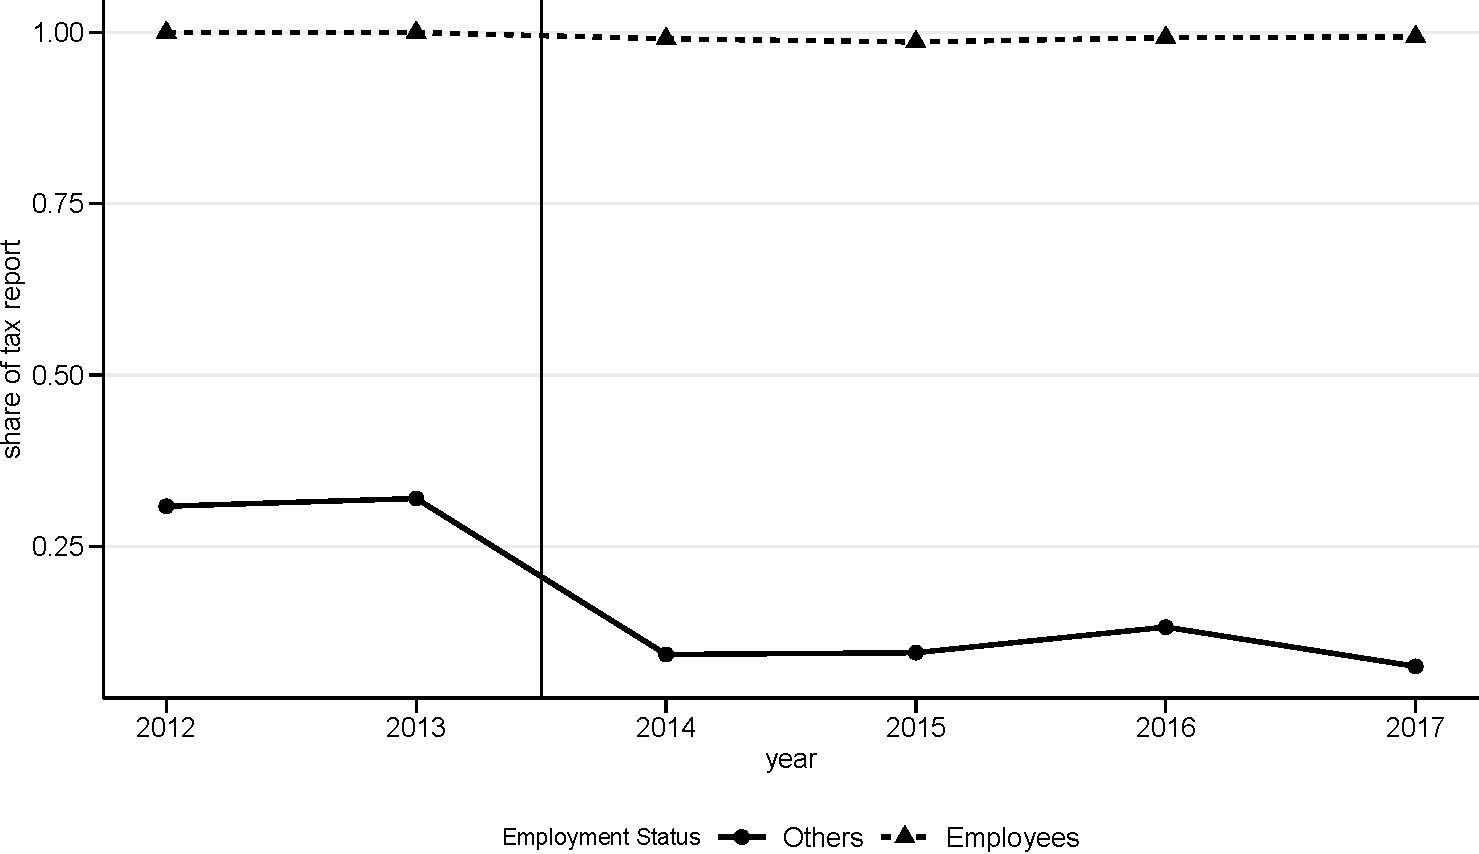
\includegraphics{C:/Users/vge00/Desktop/NASTAB/paper/draft_files/figure-latex/DeductByEmployee-1} 

}

\caption{Proportion of declaring a tax relief Grouped by Employment Status. Notes: We restrict sample to those who donated.}\label{fig:DeductByEmployee}
\end{figure}

\hypertarget{results-1}{%
\subsection{Results}\label{results-1}}

Table \ref{tab:stage1Report} shows estimation results of the first stage.
As a result, the employed dummy is strongly positively correlated with declaring a tax relief.
In any specification, employed dummy increases the probability of declaration by more than 45 percentage points.
Moreover, the ratio of coefficient to standard error is greater than nine.
This implies that the F-statistics of the instrument is greater than 81 for any specification.
Thus, our panel IV method does not have a weak instrument problem.
For the second stage, we obtain the predicted value of \(R_{it}\), using the model (3).

\begin{table}

\caption{\label{tab:stage1Report}First-Stage Result: Effect of Employee on Declaration}
\centering
\fontsize{9}{11}\selectfont
\begin{threeparttable}
\begin{tabular}[t]{lccc}
\toprule
 & (1) & (2) & (3)\\
\midrule
employee & 0.508*** & 0.464*** & 0.457***\\
 & (0.047) & (0.049) & (0.050)\\
Individual and time FE & Y & Y & Y\\
log(income) & N & Y & Y\\
Age & N & Y & Y\\
Year x Education & N & Y & Y\\
Year x Gender & N & Y & Y\\
Year x Resident Area & N & Y & Y\\
Year x Dummy of industry & N & N & Y\\
F-stat of a dummy of employee & 117.23 & 90.55 & 84.96\\
N & 11088 & 11085 & 10942\\
Adjusted R-squared & 0.918 & 0.919 & 0.920\\
\bottomrule
\end{tabular}
\begin{tablenotes}
\item Notes: $^{*}$ $p < 0.1$, $^{**}$ $p < 0.05$, $^{***}$ $p < 0.01$. Standard errors are clustered at individual level. When controlling age, we alson include its squared term.
\end{tablenotes}
\end{threeparttable}
\end{table}

Table \ref{tab:OverallReport} reports overall elasticities controlling the self-selection of the tax report.
The estimated elasticities are similar value to the benchmark results shown in Table \ref{tab:MainOverall}.
When we only include individual and time fixed effects, the overall elasticity is -2.364.
When we control the same covariates as the model (5) in Table \ref{tab:MainOverall},
the overall elasticity is -1.710.
These values are statistically significant,
and slightly more elastic than the benchmark results
(see the column (1) and (5) in Table \ref{tab:MainOverall}).
Since those who did not apply for the Declaration did not receive the tax incentive actually,
these results can be naturally interpretable.
Furthermore, when we control the interaction term between year dummies and industry dummies,
the result does not change.

In Table \ref{tab:IntensiveReport} and Table \ref{tab:ExtensiveReport},
we show the intensive-margin elasticity and the extensive-margin elasticity.
The estimated elasticities are quite similar to the benchmark results
shown in Table \ref{tab:MainIntensive} and Table \ref{tab:MainExtensive}.
Column (2) of Table \ref{tab:IntensiveReport} uses the same covariates as in the benchmark result,
the estimated value is similar to the benchmark one (the fifth column of Table \ref{tab:MainIntensive}).
About the extensive-margin elasticity,
column (2) of Table \ref{tab:ExtensiveReport} uses the same covariates as in the benchmark result,
the estimated value is similar to the benchmark one (the fifth column of Table \ref{tab:MainExtensive}).
When we further control for the interaction between year dummies and industry dummies,
we can obtain similar estimated values.

We estimate the true price effect using panel IV.
As a result, we obtain similar results to the benchmark results
shown in Table \ref{tab:MainOverall}, Table \ref{tab:MainIntensive}, and Table \ref{tab:MainExtensive}.

\begin{table}

\caption{\label{tab:OverallReport}Second-Stage Result (Overall Price Elasticity)}
\centering
\fontsize{9}{11}\selectfont
\begin{threeparttable}
\begin{tabular}[t]{lccc}
\toprule
 & (1) & (2) & (3)\\
\midrule
Propensity of Deduction x log(first price) & -2.364*** & -1.710*** & -1.603***\\
 & (0.401) & (0.447) & (0.466)\\
Individual and time FE & Y & Y & Y\\
log(income) & N & Y & Y\\
Age & N & Y & Y\\
Year x Education & N & Y & Y\\
Year x Gender & N & Y & Y\\
Year x Resident Area & N & Y & Y\\
Year x Dummy of industry & N & N & Y\\
N & 16946 & 16946 & 16946\\
Adjusted R-squared & 0.511 & 0.513 & 0.514\\
\bottomrule
\end{tabular}
\begin{tablenotes}
\item Notes: $^{*}$ $p < 0.1$, $^{**}$ $p < 0.05$, $^{***}$ $p < 0.01$. Standard errors are clustered at individual level. When controlling age, we alson include its squared term. Propensity of Deduction is the predicted value of $R_{it}$ calculated by the model (3) in Table \ref{tab:stage1Report}.
\end{tablenotes}
\end{threeparttable}
\end{table}

\begin{table}

\caption{\label{tab:IntensiveReport}Second-Stage Result (Intensive-Margin Price Elasticity)}
\centering
\fontsize{9}{11}\selectfont
\begin{threeparttable}
\begin{tabular}[t]{lccc}
\toprule
 & (1) & (2) & (3)\\
\midrule
Propensity of Report x log(first price) & -1.161*** & -0.947*** & -0.987***\\
 & (0.284) & (0.318) & (0.342)\\
Individual and time FE & Y & Y & Y\\
log(income) & N & Y & Y\\
Age & N & Y & Y\\
Year x Education & N & Y & Y\\
Year x Gender & N & Y & Y\\
Year x Resident Area & N & Y & Y\\
Year x Dummy of industry & N & N & Y\\
N & 5840 & 5840 & 5840\\
Adjusted R-squared & 0.696 & 0.698 & 0.697\\
\bottomrule
\end{tabular}
\begin{tablenotes}
\item Notes: $^{*}$ $p < 0.1$, $^{**}$ $p < 0.05$, $^{***}$ $p < 0.01$. Standard errors are clustered at individual level. When controlling age, we alson include its squared term. Propensity of Deduction is the predicted value of $R_{it}$ calculated by the model (3) in Table \ref{tab:stage1Report}.
\end{tablenotes}
\end{threeparttable}
\end{table}

\begin{table}

\caption{\label{tab:ExtensiveReport}Second-Stage Result (Extensive-Margin Price Elasticity)}
\centering
\fontsize{9}{11}\selectfont
\begin{threeparttable}
\begin{tabular}[t]{lccc}
\toprule
 & (1) & (2) & (3)\\
\midrule
Propensity of Deduction x log(first price) & -0.506*** & -0.347*** & -0.319***\\
 & (0.090) & (0.104) & (0.110)\\
 &  &  & \\
Implied price elasticity & -1.469*** & -1.008*** & -0.926***\\
 & (0.262) & (0.301) & (0.320)\\
Individual and time FE & Y & Y & Y\\
log(income) & N & Y & Y\\
Age & N & Y & Y\\
Year x Education & N & Y & Y\\
Year x Gender & N & Y & Y\\
Year x Resident Area & N & Y & Y\\
Year x Dummy of industry & N & N & Y\\
N & 16946 & 16946 & 16946\\
Adjusted R-squared & 0.426 & 0.427 & 0.428\\
\bottomrule
\end{tabular}
\begin{tablenotes}
\item Notes: $^{*}$ $p < 0.1$, $^{**}$ $p < 0.05$, $^{***}$ $p < 0.01$. Standard errors are clustered at individual level. When controlling age, we alson include its squared term. Propensity of Deduction is the predicted value of $R_{it}$ calculated by the model (3) in Table \ref{tab:stage1Report}. The implied extensive-marign price elasticity is evaluated at the sample mean of $D_{ijt}$.
\end{tablenotes}
\end{threeparttable}
\end{table}

\hypertarget{conclusions}{%
\section{Conclusions}\label{conclusions}}

In this paper, we investigate the giving price elasticity using South Korean panel data. As a result, we obtain the following findings.

Firstly, our baseline estimation shows that the giving price elasticity in Korea is around -1 even if we take into account the existence of the undeclared charitable giving. Since the literature of the tax expenditure for charitable giving suggests that the price elasticity is around -1, the result suggests that the effect coming from the existence of the undeclared charitable giving cost may be limited.

Secondly, we find that the estimated price elasticity using the effective giving price takes the similar values from the estimated elasticity in the extant research. It implies that the effect from the declaration cost, which has been ignored, is not so large. Moreover, as well as the baseline result, this result shows that the price elasticity is around -1, which derives the same conclusions as the baseline result.

From the results, we firstly show the giving price elasticity in Korea. However, many things to be considered are remaining. To understand the giving behavior and to contribute the policy making, more sophisticated research is needed.

\clearpage

\hypertarget{references}{%
\section*{References}\label{references}}
\addcontentsline{toc}{section}{References}

\hypertarget{refs}{}
\begin{CSLReferences}{1}{0}
\leavevmode\vadjust pre{\hypertarget{ref-Almunia2020}{}}%
Almunia, M., Guceri, I., Lockwood, B., Scharf, K., 2020. More giving or more givers? The effects of tax incentives on charitable donations in the UK. Journal of Public Economics 183. doi:\href{https://doi.org/10.1016/j.jpubeco.2019.104114}{10.1016/j.jpubeco.2019.104114}

\leavevmode\vadjust pre{\hypertarget{ref-Auten2002}{}}%
Auten, G.E., Sieg, H., Clotfelter, C.T., 2002. Charitable giving, income, and taxes: An analysis of panel data. American Economic Review 92, 371--382.

\leavevmode\vadjust pre{\hypertarget{ref-Bakija2011}{}}%
Bakija, J., Heim, B.T., 2011. How does charitable giving respond to incentives and income? New estimates from panel data. National Tax Journal 64, 615--650. doi:\href{https://doi.org/10.17310/ntj.2011.2S.08}{10.17310/ntj.2011.2S.08}

\leavevmode\vadjust pre{\hypertarget{ref-Fack2010}{}}%
Fack, G., Landais, C., 2010. Are tax incentives for charitable giving efficient? Evidence from france. American Economic Journal - Economic Policy 2, 117--141. doi:\href{https://doi.org/10.1257/pol.2.2.117}{10.1257/pol.2.2.117}

\leavevmode\vadjust pre{\hypertarget{ref-Fack2016}{}}%
Fack, G., Landais, C., 2016. The effect of tax enforcement on tax elasticities: Evidence from charitable contributions in france. Journal of Public Economics 133, 23--40. doi:\url{https://doi.org/10.1016/j.jpubeco.2015.10.004}

\leavevmode\vadjust pre{\hypertarget{ref-Gillitzer2018}{}}%
Gillitzer, C., Skov, P.E., 2018. {The use of third-party information reporting for tax deductions: evidence and implications from charitable deductions in Denmark}. Oxford Economic Papers 70, 892--916. doi:\href{https://doi.org/10.1093/oep/gpx055}{10.1093/oep/gpx055}

\leavevmode\vadjust pre{\hypertarget{ref-Randolph1995}{}}%
Randolph, W.C., 1995. Dynamic income, progressive taxes, and the timing of charitable contributions. Journal of Political Economy 103, 709--738. doi:\href{https://doi.org/10.1086/262000}{10.1086/262000}

\leavevmode\vadjust pre{\hypertarget{ref-Rehavi2013}{}}%
Rehavi, M., Shack, D., 2013. Partial reporting: An example from charitable giving. Working paper of University of British Columbia.

\leavevmode\vadjust pre{\hypertarget{ref-Saez2004}{}}%
Saez, E., 2004. The optimal treatment of tax expenditures. Journal of Public Economics 88, 2657--2684. doi:\href{https://doi.org/10.1016/j.jpubeco.2003.09.004}{10.1016/j.jpubeco.2003.09.004}

\leavevmode\vadjust pre{\hypertarget{ref-Zeldow2019}{}}%
Zeldow, B., Hatfield, L.A., 2021. Confounding and regression adjustment in difference-in-differences studies. Health Services Research n/a. doi:\url{https://doi.org/10.1111/1475-6773.13666}

\end{CSLReferences}

\end{document}
